\documentclass[ucs, notheorems, handout]{beamer}

\usetheme[numbers,totalnumbers, nologo]{Statmod}
\usefonttheme[onlymath]{serif}
\setbeamertemplate{navigation symbols}{}

\mode<handout> {
	\usepackage{pgfpages}
	%\setbeameroption{show notes}
	%\pgfpagesuselayout{2 on 1}[a4paper, border shrink=5mm]
	\setbeamercolor{note page}{bg=white}
	\setbeamercolor{note title}{bg=gray!10}
	\setbeamercolor{note date}{fg=gray!10}
}

\usepackage[utf8x]{inputenc}
\usepackage[T2A]{fontenc}
\usepackage[russian]{babel}
\usepackage{tikz}
\usepackage{ragged2e}

\newtheorem{theorem}{Теорема}
\newtheorem*{definition}{Определение}
\newtheorem{lemma}{Лемма}
\usepackage{amsmath}
\usepackage{amsthm}
\usepackage{bm}
\usepackage{bbold}

\usepackage{pgfplots}
\pgfplotsset{compat=1.9}

\usepackage{graphicx}
%\usepackage[usenames]{color}
%\usepackage{colortbl}

%\newtheorem{theorem}{Теорерма}
\newtheorem{corollary}[theorem]{Следствие}
%\newtheorem{lemma}[theorem]{Лемма}
\newtheorem{observation}[theorem]{Observation}
\newtheorem{proposition}[theorem]{Предложение (Swanson)}
\newtheorem{proposition2}[theorem]{Предложение}
%\newtheorem{definition}[theorem]{Определение}
\newtheorem{claim}[theorem]{Утверждение}
\newtheorem{fact}[theorem]{Факт}
\newtheorem{assumption}[theorem]{Предположение}
\newtheorem{alg}{Алгоритм}
\newtheorem{zam}{Замечание}

\newtheorem{example}{Пример}[section]

\newenvironment{Proof}{\par\noindent{\bf Доказательство.}}{\hfill$\scriptstyle\blacksquare$}
\newenvironment{ex}{\par\noindent{\bf Пример.}}{}
\newenvironment{pr1}{\par\noindent{\bf Дано:}}{}
\newenvironment{pr2}{\par\noindent{\bf Шаги:}}{}
\newenvironment{pr3}{\par\noindent{\bf Результат:}}{}

\DeclareMathOperator{\tr}{tr}
\DeclareMathOperator{\F}{\mathsf{F}}

\title[Замена непрерывного распределения]{Замена непрерывного распределения на дискретное для применения на практике}
\author[Нагуманова~К. И.]{ Нагуманова Карина Ильнуровна, 19Б.04-мм}

\date{\tiny{Санкт-Петербург\\ 2023г.}}
\institute[Санкт-Петербургский Государственный Университет]{%
	\small
	Санкт-Петербургский государственный университет\\
	Прикладная математика и информатика\\
	%Вычислительная стохастика и статистические модели\\
	\vspace{1.25cm}}
\begin{document}
	
	\begin{frame}
		\titlepage
		\note{Научный руководитель  д.ф.-м.н., доцент Голяндина Н.\,Э.,\\
			кафедра статистического моделирования}
	\end{frame}

\begin{frame}{Введение}
	В практических задачах нередко требуется заменить непрерывное распределение на
	дискретное с сохранением математического ожидания и дисперсии. Одним из методов
	нахождения такого распределения для трехточечной аппроксимации нормального распределения является \textcolor{blue}{\hbox{\textbf{метод Свонсона}}}.
	
	\bigskip
	
	Однако в ряде областей, например, в нефтяной промышленности, общепринятым распределением, описывающим запасы нефти, является логнормальное распределение. 
	Соответственно, реальной задачей является аппроксимация логнормального распределения. При этом здесь тоже применим метод Свонсона, потому что логнормальное распределение можно свести к нормальному.
\end{frame}

\begin{frame}{Введение}
	
	Аппроксимируемые случайные величины складывают и умножают.
	
	\bigskip
	
	\textcolor{blue}{\hbox{Пример перемножения:}} используем площадь дренирования пласта, среднюю чистую толщину и коэффициент извлечения углеводородов. При перемножении этих параметров получаем количество резервов нефти.
	
	\bigskip
	
	\textcolor{blue}{\hbox{Пример сложения:}} зная запасы нефти в разных скважинах, нужно оценить суммарные запасы.
	
	\bigskip
	
	\textcolor{red}{\textbf{Задача:}} находить аппроксимацию суммы и произведения по аппроксимациям исходных случайных величин.
	
\end{frame}

\begin{frame}{Введение}
	\textbf{План работы.}
	\begin{enumerate}
		\item Рассмотреть общий подход к трехточечной аппроксимации.
		\item Рассмотреть трехточечную аппроксимацию нормального распределения, в целом метод Свонсона и вывод правила 30-40-30.
		\item Рассмотреть трехточечную аппроксимацию логнормального распределения и её  свойства.
		\item Построить алгоритм аппроксимации произведения двух логнормальных распределений.
		\item Построить алгоритм аппроксимации суммы двух логнормальных распределений.
	\end{enumerate}
\end{frame}

\begin{frame}{Часть 1: Общий подход к трехточечной аппроксимации}
	$\xi$ "--- непрерывная случайная величина  \[m = \mathbf E(\xi), \quad\quad s^{2} = \mathbf D(\xi)\]  $F(x)$ "--- функция распределения,
	$x_{\pi_{1}}$, $x_{\pi_{2}}$, $x_{\pi_{3}}$ "--- квантили $\xi$.
	
	$\tilde{\xi}$ "--- случайная дискретная величина 
	
	\[\tilde{\xi}:\quad\begin{pmatrix} 
		x_{\pi_{1}}&x_{\pi_{2}}&x_{\pi_{3}}\\ 
		p_{1} &  p_{2}  & p_{3}
	\end{pmatrix}\]
	
	\[\tilde{m} = \mathbf E(\tilde{\xi}), \quad\quad \tilde{s}^{2} = \mathbf D(\tilde{\xi})\]
	\textcolor{red}{\textbf{Задача:}} аппроксимировать распределение случайной величины $\xi$ дискретным распределением $\tilde{\xi}$, то есть найти $p_{1}$, $p_{2}$, $p_{3}$ такие, что 
	\begin{equation*}
		p_{1} + p_{2} + p_{3} = 1, \label{1}
	\end{equation*}
	\begin{equation*}
		\tilde{m} = p_{1}x_{\pi_{1}} + p_{2}x_{\pi_{2}} + p_{3}x_{\pi_{3}} = m, \label{2}
	\end{equation*}
	\begin{equation*}
		\tilde{s}^{2} = p_{1} x_{\pi_{1}}^{2} + p_{2} x_{\pi_{2}}^{2} + p_{3} x_{\pi_{3}}^{2} - m^{2} = s^{2}. \label{3}
	\end{equation*}
	
	
	\note{Постановка задачи в общем виде. Основные обозначения.}
\end{frame}

\begin{frame}{Часть 1: Общий подход к трехточечной аппроксимации}
	\begin{proposition}\label{pr1}
		Пусть верно 
		\begin{equation*}
			\begin{pmatrix} 
				1&1&1\\ 
				\hat{x}_{\pi_{1}}~~ &  \hat{x}_{\pi_{2}}~~  & \hat{x}_{\pi_{3}} \\ 
				\hat{x}_{\pi_{1}}^{2}~~&\hat{x}_{\pi_{2}}^{2}~~  &\hat{x}_{\pi_{3}}^{2}
			\end{pmatrix}
			\begin{pmatrix}p_{1}\\p_{2}\\ p_{3}\end{pmatrix}= \begin{pmatrix}1\\0\\1 \end{pmatrix},\label{4}
		\end{equation*}
	где $\hat{x}_{\pi_{i}} = \hat{\F}^{-1}(\pi_{i})$, $\hat{\F}(y)$ "--- функция распределения $\displaystyle{\hat{\xi} = \frac{\xi-m}{s}}$. Тогда $m=\tilde{m}$ и $s^{2} = \tilde{s}^{2}$.
	\end{proposition}
	
	%\bigskip
	Если $\xi\sim N(\mu, \sigma) $ имеет нормальное распределение, то
	$\hat{\xi}$ имеет нормальное стандартное распределение, поэтому можно написать систему, которая не зависит от $\mu$ и $\sigma$.
\end{frame}


\begin{frame}{Часть 2: Аппроксимация нормального распределения}
	\begin{equation*}
		\begin{pmatrix} 1&1&1\\ 
			\Phi^{-1}(\pi)~~ &  0~~  & -\Phi ^{-1}(\pi) \\ 
			\Phi ^{-1}(\pi)^{2}~~& 0~~  &\Phi ^{-1}(\pi)^{2}
		\end{pmatrix} 
		\begin{pmatrix}p_{\pi}\\p_{0.5}\\ p_{1-\pi}\end{pmatrix}= \begin{pmatrix}1\\0\\1\end{pmatrix}.
	\end{equation*}
	
	\begin{proposition}\label{pr7}
		$\xi\sim N(\mu, \sigma)$, пусть верно 
		\begin{equation*}
			\begin{cases}
				p_{\pi} = p_{1-\pi}=\displaystyle{\frac{\delta}{2}},\\ 
				p_{0.5}=1-\delta,
			\end{cases}\label{7}
		\end{equation*}
		где $\delta  = \displaystyle{\frac{1}{\Phi ^{-1}(\pi)^{2}}}$. Тогда $m=\tilde{m}$ и $s^{2} = \tilde{s}^{2}$.
	\end{proposition}
\end{frame}

\begin{frame}{Часть 2: Аппроксимация нормального распределения}
	Рассмотрим частный случай $\pi = 0.1$, имеем 
	$$\Phi ^{-1}(0.1) = -\Phi ^{-1}(0.9) \approx  -1.28, \qquad \Phi ^{-1}(0.5) = 0. $$
	\begin{equation*}
		\begin{cases}
			p_{1}\approx 0.305, \\ 
			p_{2}\approx 0.390,  \\ 
			p_{3}\approx 0.305.
		\end{cases}
	\end{equation*}
	
	Эти вероятности примерно равны 0.3, 0.4, 0.3, поэтому это правило называют \textcolor{blue}{\hbox{\textbf{правилом 30-40-30}}}.
	
\end{frame}	

\begin{frame}{Часть 3: Связь логнормального распределения с нормальным}
	Моменты $m$, $s^{2}$ логнормального распределения выражаются через моменты $\mu$, $\sigma ^{2}$ соответствующего нормального распределения:
	\begin{equation*}
		m = \exp\left( \mu+\frac{\sigma ^{2}}{2}\right) ,
	\end{equation*} \label{10}
	\begin{equation*}
		s^{2} = m^{2}(\exp(\sigma^{2})-1).
	\end{equation*} \label{11}
	Параметр $\sigma$ выражается как
	\begin{equation*}
		\displaystyle{\sigma = \dfrac{\log\left(\dfrac{x_{\pi_{j}}}{x_{\pi_{i}}}\right)}{\Phi ^{-1}(\pi_{j}) - \Phi ^{-1}(\pi_{i})}}, \quad \quad i\neq j.
	\end{equation*} \label{13}
	Значение $\sigma$ одинаковое для любых пар i и j.
	\begin{equation*}
		\mu = \log(x_{\pi_{i}}) - \sigma\Phi ^{-1}(\pi_{i}).
	\end{equation*}
	Результат не зависит от i.
	%\textbf{\textit{Доказательство:}}
\end{frame}

	
	\begin{frame}{Часть 3: Аппроксимация логнормального распределения}
			\begin{pr1}
				квантили $x_{\pi_{1}}, x_{\pi_{2}}, x_{\pi_{3}}$ логнормальной случайной величины $\eta$, $\ln(\eta) \sim N(\mu, \sigma)$.
			\end{pr1}
		
		\bigskip
		
			\begin{enumerate}
				\item Вычисляем значения мат. ожидания $m$ и дисперсии $s^{2}$ случайной величины $\eta$, используя известные $x_{\pi_{1}}, x_{\pi_{2}}, x_{\pi_{3}}$.
				\item Выражаем параметры $\mu$ и $\sigma$ мат. ожидание и дисперсию соответствующего нормального распределения через параметры $m$ и $s^{2}$ логнормального распределения
				\item С помощью системы уравнений из метода для нормального распределения находим значения вероятностей $p_{1}$, $p_{2}$, $p_{3}$.
			\end{enumerate}
		\bigskip
			\begin{pr3}\end{pr3} вероятности $p_{1}$, $p_{2}$, $p_{3}$ для $x_{\pi_{1}}, x_{\pi_{2}}, x_{\pi_{3}}$ случайной величины $\tilde{\xi}$.
		
		\note{Способ аппроксимации логнормального распределения через переход к нормальному.}
	\end{frame}

\begin{frame}{Часть 3: Условие на параметр $\sigma$}
	Мною доказаны следующие предложения.
		\begin{proposition2}
		Положительные вероятности $p_{1}$, $p_{2}$, $p_{3}$ для аппроксимации логнормальной случайной величины $\eta$ существуют только при условии \[\exp(\sigma^{2})+\exp(-\sigma^{2})-\exp\left( -\dfrac{\sigma^{2}}{2}\right) 
		(\exp(c\sigma)+\exp(-c\sigma))\leq 0,\] 
		где $c = \Phi^{-1}(\pi)$.
		%(при $\sigma\leq 0.6913$, $\gamma_{3}\leq 2.8278$ примерно).
	\end{proposition2}
	
	\begin{proposition2}
		При уменьшении значения $\pi$ ограничение на $\sigma$ становится слабее, то есть диапазон значений $\sigma$ увеличивается.
	\end{proposition2}

\end{frame}

\begin{frame}{Часть 3: Варианты постановки задачи}
	\textbf{Задача:} имеются квантили $x_{\pi}$, $x_{0.5}$, $x_{1-\pi}$ логнормальной случайной величины $\eta$. Нужно уметь считать $m$ и $s^{2}$.
	
	\begin{enumerate}
		\item Используя значения двух квантилей, найти значения параметров $\mu$ и $\sigma$ нормальной случайной величины $\ln(\eta)\sim N(\mu, \sigma)$. Через них вычислить значения $m$ и $s^{2}$.
		\item Найти значения $p_{1}$, $p_{2}$, $p_{3}$ такие, что 
		\begin{equation*}
			p_{1}x_{\pi_{1}} + p_{2}x_{\pi_{2}} + p_{3}x_{\pi_{3}} = m, \label{2}
		\end{equation*}
		\begin{equation*}
			p_{1} x_{\pi_{1}}^{2} + p_{2} x_{\pi_{2}}^{2} + p_{3} x_{\pi_{3}}^{2} - m^{2} = s^{2}.
		\end{equation*}
		Если $p_{1}$, $p_{2}$, $p_{3}$ положительные, то рассматривается аппроксимация дискретной $\tilde{\xi}$, у которой $\tilde{m} = m$ и $\tilde{s}^{2}=s^{2}$.
		Если не все положительные, то можно воспринимать задачу формально, как поиск коэффициентов линейной комбинации $x_{\pi}$, $x_{0.5}$, $x_{1-\pi}$. 
	\end{enumerate}
\end{frame}

\begin{frame}{Часть 3: Точность метода Свонсона для логнормального распределения}
	\textbf{Проблема:} метод Свонсона, применяемый к нормальному распределению, используют для логнормального распределения.
	
	\textbf{Вопрос:} какова точность аппроксимации $m$ и $s^{2}$?
	
	\begin{proposition2}\label{pr5}
		Ошибка аппроксимации мат.ожидания логнормального распределения по методу Свонсона, применяемому к нормальному распределению, равна
		\[\dfrac{\mid m - \widetilde{m} \mid}{m} = \biggl| \exp\left( \dfrac{\sigma^{2}}{2}\right)  - \dfrac{1}{2 c^{2}}\times\]\[\times(\exp(c\sigma)-1 +\exp(-c\sigma)) + 1 \biggr|/\exp\left(\dfrac{\sigma^{2}}{2}\right),\]
		где $c = \Phi^{-1}(\pi)$, и не зависит от параметра $\mu$.
	\end{proposition2}
\end{frame}

\begin{frame}{Часть 3: Точность метода Свонсона для логнормального распределения}
	\begin{proposition2}\label{pr6}
		Ошибка аппроксимации дисперсии логнормального распределения по методу Свонсона, применяемому к нормальному распределению, равна
		\[\dfrac{\mid s^{2} - \widetilde{s}^{2} \mid}{s^{2}} = \biggl|\exp(\sigma^{2})(\exp(\sigma^{2}-1)) -\]\[- \dfrac{1}{2c^{2}}\exp(-2c\sigma)- \left( 1- \dfrac{1}{c^{2}}\right) \exp(2c\sigma)+\]\[+ \left( \dfrac{1}{2c^{2}}(\exp(c\sigma)-1+\exp(-c\sigma)) + 1\right) ^{2}\biggr| /\exp(\sigma^{2})(\exp(\sigma^{2}-1)),\]
		где $c = \Phi^{-1}(\pi)$, и не зависит от параметра $\mu$.
		
		%\mid
		
	\end{proposition2}
\end{frame}

\begin{frame}{Часть 3: Точность метода Свонсона для логнормального распределения}

	\begin{figure}[h]
	\begin{center}
		\begin{minipage}[h]{0.6\linewidth}
			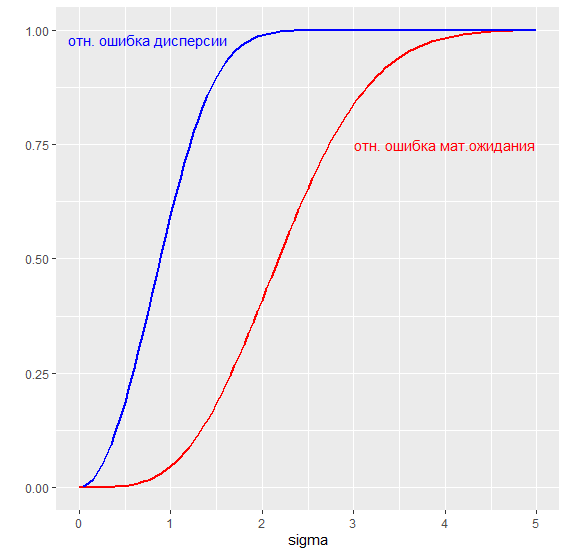
\includegraphics[width=1\linewidth]{img/par_new2.jpg}
			\caption{Относительная ошибка аппроксимации мат.ож. и дисперсии} %% подпись к рисунку
			\label{ris:image2} %% метка рисунка для ссылки на него
		\end{minipage}
		
	\end{center}
\end{figure}

%Видим, что при $\sigma\leq1.5$ ошибка аппроксимации мат.ожидания меньше $12\%$. 
%Видим, что при $\sigma\leq1.5$ ошибка аппроксимации дисперсии может достигать $80\%$. 
	
\end{frame}
	
	\begin{frame}{Часть 4: Произведение двух логнормальных распределений}
		Рассмотрим две логнормальные случайные величины
		\begin{itemize}
			\item $\ln(\xi_{1}) \sim N(\mu_{1}, \sigma _{1}^{2})$,
			\item $\ln(\xi_{2}) \sim N(\mu_{2}, \sigma _{2}^{2})$,
		\end{itemize}
		которые заданы своими квантилями
		\begin{itemize}
			\item $x_{\pi}$, $x_{0.5}$, $x_{1-\pi}$ "--- симметричные квантили $\xi_{1}$,
			\item $y_{\pi}$, $y_{0.5}$, $y_{1-\pi}$ "--- симметричные квантили $\xi_{2}$.
		\end{itemize}
	
		\bigskip
		
		\textbf{Задача:} аппроксимировать непрерывную случайную величину $\eta = \xi_{1}\xi_{2}$ дискретной, то есть найти квантили вида $z_{\pi}$, $z_{0.5}$, $z_{1-\pi}$.
		
	\end{frame}

	\begin{frame}{Часть 4: Произведение двух логнормальных распределений}
	
		\begin{proposition}
		Зная квантили $x_{\pi}$, $x_{0.5}$, $x_{1-\pi}$ случайной величины $\xi_{1}$ и квантили $y_{\pi}$, $y_{0.5}$, $y_{1-\pi}$ случайной величины $\xi_{2}$ можно найти квантили $z_{\pi}$, $z_{0.5}$, $z_{1-\pi}$ случайной величины $\xi_{1}\xi_{2}$, как
		
		\begin{equation*}
			z_{\pi}=\exp(b\Phi^{-1}(\pi)+a),
		\end{equation*}
		\begin{equation*}
			z_{0.5}=x_{0.5}y_{0.5},
		\end{equation*}
		\begin{equation*}
			z_{1-\pi}=\exp(b\Phi^{-1}(1-\pi)+a),
		\end{equation*}
		
		где $a$ и $b$ такие, что прямая $y=\dfrac{x-a}{b}$, проходит через точки $(\ln(x_{\pi}y_{\pi}), t)$ и $(\ln(x_{0.5}y_{0.5}),0)$, где
		\begin{equation*}
			t = \frac{\Phi^{-1}(\pi)((\ln(x_{0.5})+\ln(y_{0.5}))-(\ln(x_{\pi})+\ln(y_{\pi})))}{\sqrt{(\ln(x_{0.5})-\ln(x_{\pi}))^{2}+(\ln(y_{0.5})-\ln(y_{\pi}))^{2}}}. 
		\end{equation*}
	\end{proposition}
\end{frame}



\begin{frame}{Часть 5: Сумма двух логнормальных распределений }
	
		Рассмотрим сумму двух логнормальных случайных величин.
	\begin{equation*}
		\ln(\xi_{1}) \sim N(\mu_{1}, \sigma _{1}^{2}),
	\end{equation*}
	\begin{equation*}
		\ln(\xi_{2}) \sim N(\mu_{2}, \sigma _{2}^{2}),
	\end{equation*}
	\begin{equation*}
		\xi = \xi_{1}+\xi_{2}.
	\end{equation*}
	$\xi_{1}$ и $\xi_{2}$ заданы своими квантилями.
	\bigskip
	
	Поставим задачу аппроксимации суммы логнормальным распределением $\ln(\eta)\sim N(\mu, \sigma)$, так как нужно рассматривать сумму не обязательно двух, а произвольного числа случайных величин. 
	
	\bigskip
	
	\textbf{Задача:} найти квантили $z_{\pi}$, $z_{0.5}$, $z_{1-\pi}$ случайной величины $\eta$.
	
	\bigskip
	
	Далее уже знаем, как вычислить вероятности $p_{1}$, $p_{2}$, $p_{3}$ такие, что $m = \tilde{m}$  и $s^{2} = \tilde{s}^{2}$.

	
\end{frame}

\begin{frame}{Часть 5: Сумма двух логнормальных распределений}
	
	\begin{pr1}
		Квантили $x_{\pi}$, $x_{0.5}$, $x_{1-\pi}$ "--- квантили $\xi_{1}$, $y_{\pi}$, $y_{0.5}$, $y_{1-\pi}$ "--- квантили $\xi_{2}$.
	\end{pr1}
	\begin{enumerate}
		\item $x_{\pi}$, $x_{0.5}$, $x_{1-\pi}$ $\rightarrow$  $\mu_{1}$, $\sigma_{1}$
		\item $y_{\pi}$, $y_{0.5}$, $y_{1-\pi}$ $\rightarrow$ $\mu_{2}$, $\sigma_{2}$
		\item $\mu_{i}$, $\sigma_{i}$ $\rightarrow$ $m_{i}$, $s_{i}^{2}$
		\item $m = m_{1}+m_{2}$
		\item $s^{2}=s_{1}^{2} + s_{2}^{2}$
		\item $m$, $s^{2}$ $\rightarrow$ $\mu$, $\sigma$
		\item $\mu$, $\sigma$ $\rightarrow$ $z_{\pi}$, $z_{0.5}$, $z_{1-\pi}$
		\item $z_{\pi}$, $z_{0.5}$, $z_{1-\pi}$ $\rightarrow$ $p_{1}$, $p_{2}$, $p_{3}$
		
	\end{enumerate}
\begin{pr3}\end{pr3} вероятности $p_{1}$, $p_{2}$, $p_{3}$ для квантилей $z_{\pi_{1}}, z_{\pi_{2}}, z_{\pi_{3}}$ случайной величины $\xi_{1} + \xi_{2}$.
	
\end{frame}
	

\begin{frame}{Часть 5: Сумма двух логнормальных распределений. Точность аппроксимации }
	
	Oшибки аппроксимации квантилей $q_{10}$, $q_{50}$, $q_{90}$ случайной величины $\xi$ равны
\[\dfrac{\left| q_{10} - z_{10}\right|}{q_{10}}, \quad\quad \dfrac{\left| q_{50} - z_{50}\right|}{q_{50}}, \quad\quad \dfrac{\left| q_{90} - z_{90}\right|}{q_{90}},\] где
\[z_{100p} = F_{\eta}^{-1}(p) = \exp(\mu+\sigma\sqrt{2}\mathrm{erf}^{-1}(2p-1)).\]
Значение квантилей $q_{i}$ выражаются как $q_{100p} = F_{\xi}^{-1}(p)$, где
\[F_{\xi}(x) = \int_{0}^{x}\left( \dfrac{1}{2}+\dfrac{1}{2} \mathrm{erf}\left( \dfrac{\ln(x-y)-\mu_{1}}{\sigma_{1}\sqrt{2}}\right) \right)\times\]
\[\times \left( \dfrac{1}{\sqrt{2\pi}y\sigma_{2}}\exp\left( -\left( \dfrac{\ln(y)-\mu_{2}}{\sqrt{2}\sigma_{2}}\right) ^{2}\right) \right) dy \]
	
\end{frame}

\begin{frame}{Часть 5: Сумма двух логнормальных распределений. Точность аппроксимации }
	Рассмотрим $\ln(\xi_{1}) \sim N(4, \sigma _{1}^{2})$, $\ln(\xi_{2}) \sim N(6, \sigma _{2}^{2})$ и найдем ошибки с помощью моделирования, объемы выборок равны $10^{6}$.
	
	%\bigskip
	
	\begin{table}[ht]
		\centering
		\caption{Ошибка аппроксимации медианы ($\%$) в зависимости от $\sigma_{1}^{2}$ (строка) и $\sigma_{2}^{2}$ (столбец)}
		\begin{tabular}{rrrrrr}
			\hline
			& \textbf{0.25} & \textbf{0.75} & \textbf{1.25} & \textbf{1.75} & \textbf{2.5} \\ 
			\hline
			\textbf{0.25} & 0.58 & 0.29 & 0.89 & 2.64 & 6.41 \\ 
			\textbf{0.75} & 0.13 & 0.12 & 2.15 & 4.88 & 7.27 \\ 
			\textbf{1.25} & 0.01 & 0.83 & 2.94 & 5.58 & 10.02 \\ 
			\textbf{1.75} & 2.23 & 0.52 & 3.61 & 6.74 & 9.84 \\ 
			\textbf{2.5} & 9.15 & 3.35 & 3.25 & 6.76 & 9.89 \\ 
			\hline
		\end{tabular}
	\end{table}
	
\end{frame}

\begin{frame}{Часть 5: Сумма двух логнормальных распределений. Точность аппроксимации}
	\begin{table}[ht]
		\centering
		\caption{Ошибка аппроксимации $q_{10}$ ($\%$) в зависимости от $\sigma_{1}^{2}$ (строка) и $\sigma_{2}^{2}$ (столбец)}
		\begin{tabular}{rrrrrr}
			\hline
			& \textbf{0.25} & \textbf{0.75} & \textbf{1.25} & \textbf{1.75} & \textbf{2.5} \\
			\hline
			\textbf{0.25} & 2.35 & 13.59 & 23.93 & 33.20 & 42.75 \\ 
			\textbf{0.75} & 1.20 & 10.54 & 21.80 & 33.93 & 42.82 \\ 
			\textbf{1.25} & 3.02 & 7.03 & 18.43 & 29.49 & 40.09 \\ 
			\textbf{1.75} & 14.45 & 5.27 & 14.33 & 26.50 & 36.75 \\ 
			\textbf{2.5} & 34.70 & 11.44 & 11.10 & 23.05 & 32.84 \\ 
			\hline
		\end{tabular}
	\end{table}
	
\end{frame}

\begin{frame}{Часть 5: Сумма двух логнормальных распределений. Точность аппроксимации}
	
	\begin{table}[ht]
		\centering
		\caption{Ошибка аппроксимации $q_{90}$ ($\%$) в зависимости от $\sigma_{1}^{2}$ (строка) и $\sigma_{2}^{2}$ (столбец) }
		\begin{tabular}{rrrrrr}
			\hline
			& \textbf{0.25} & \textbf{0.75} & \textbf{1.25} & \textbf{1.75} & \textbf{2.5} \\
			\hline
			\textbf{0.25} & 1.01 & 3.00 & 4.24 & 4.10 & 3.40 \\ 
			\textbf{0.75} & 0.04 & 2.51 & 4.11 & 3.26 & 5.45 \\ 
			\textbf{1.25} & 1.44 & 1.81 & 3.29 & 3.93 & 5.82 \\ 
			\textbf{1.75} & 8.25 & 2.60 & 2.93 & 3.60 & 4.49 \\ 
			\textbf{2.5} & 18.17 & 3.00 & 3.30 & 2.44 & 4.99 \\ 
			\hline
		\end{tabular}
	\end{table}
	
\end{frame}



\begin{frame}{Часть 5: Сумма двух логнормальных распределений. Точность аппроксимации}
	
	Посчитаем значения функции $F_{\xi}(x)$ от квантилей $z_{10}$, $z_{50}$, $z_{90}$ случайной величины $\eta$. Они показывают, каким квантилем для $\xi$ являются квантили $z_{i}$. Результаты приведены в следующих таблицаx.
	
	\begin{table}[!hhh]
		\centering
		\caption{$F_{\eta}(z_{50})$ в зависимости от $\sigma_{1}^{2}$ (строка) и $\sigma_{2}^{2}$ (столбец) }
		\label{tab4}
		\begin{tabular}{rrrrr}
			\hline
			& \textbf{0.15} & \textbf{0.85} & \textbf{1.55} & \textbf{2.25} \\
			\hline
			\textbf{0.15} & 0.51 & 0.50 & 0.49 & 0.48 \\ 
			\textbf{0.85} & 0.50 & 0.50 & 0.48 & 0.47 \\ 
			\textbf{1.55} & 0.49 & 0.50 & 0.48 & 0.46 \\ 
			\textbf{2.25} & 0.40 & 0.49 & 0.48 & 0.46 \\ 
			\hline
		\end{tabular}
	\end{table}	
\end{frame}

\begin{frame}{Часть 5: Сумма двух логнормальных распределений. Точность аппроксимации}
	
	\begin{table}[!hhh]
		\centering
		\caption{$F_{\eta}(z_{10})$ в зависимости от $\sigma_{1}^{2}$ (строка) и $\sigma_{2}^{2}$ (столбец) }
		\label{tab5}
		\begin{tabular}{rrrrr}
			\hline
			& \textbf{0.15} & \textbf{0.85} & \textbf{1.55} & \textbf{2.25} \\
			\hline
			\textbf{0.15} & 0.09 & 0.06 & 0.04 & 0.02 \\ 
			\textbf{0.85} & 0.10 & 0.07 & 0.05 & 0.03 \\ 
			\textbf{1.55} & 0.05 & 0.08 & 0.06 & 0.04 \\ 
			\textbf{2.25} & 0.00 & 0.08 & 0.07 & 0.05 \\ 
			\hline
		\end{tabular}
	\end{table}
	
	\begin{table}[!hhh]
		\centering
		\caption{$F_{\eta}(z_{90})$ в зависимости от $\sigma_{1}^{2}$ (строка) и $\sigma_{2}^{2}$ (столбец)}
		\label{tab6}
		\begin{tabular}{rrrrr}
			\hline
			& \textbf{0.15} & \textbf{0.85} & \textbf{1.55} & \textbf{2.25} \\
			\hline
			\textbf{0.15} & 0.90 & 0.90 & 0.90 & 0.90 \\ 
			\textbf{0.85} & 0.90 & 0.91 & 0.91 & 0.90 \\ 
			\textbf{1.55} & 0.93 & 0.90 & 0.91 & 0.91 \\ 
			\textbf{2.25} & 0.95 & 0.91 & 0.90 & 0.91 \\ 
			\hline
		\end{tabular}
	\end{table}
\end{frame}

\begin{frame}{Часть 5: Сумма двух логнормальных распределений. Точность аппроксимации}
	
	Построим оценки плотности для $\xi$ и $\eta$, когда ошибки имеют очень маленькие значения и когда достаточно большие.
	
	\begin{figure}[h]
		\begin{center}
			\begin{minipage}[h]{0.4\linewidth}
				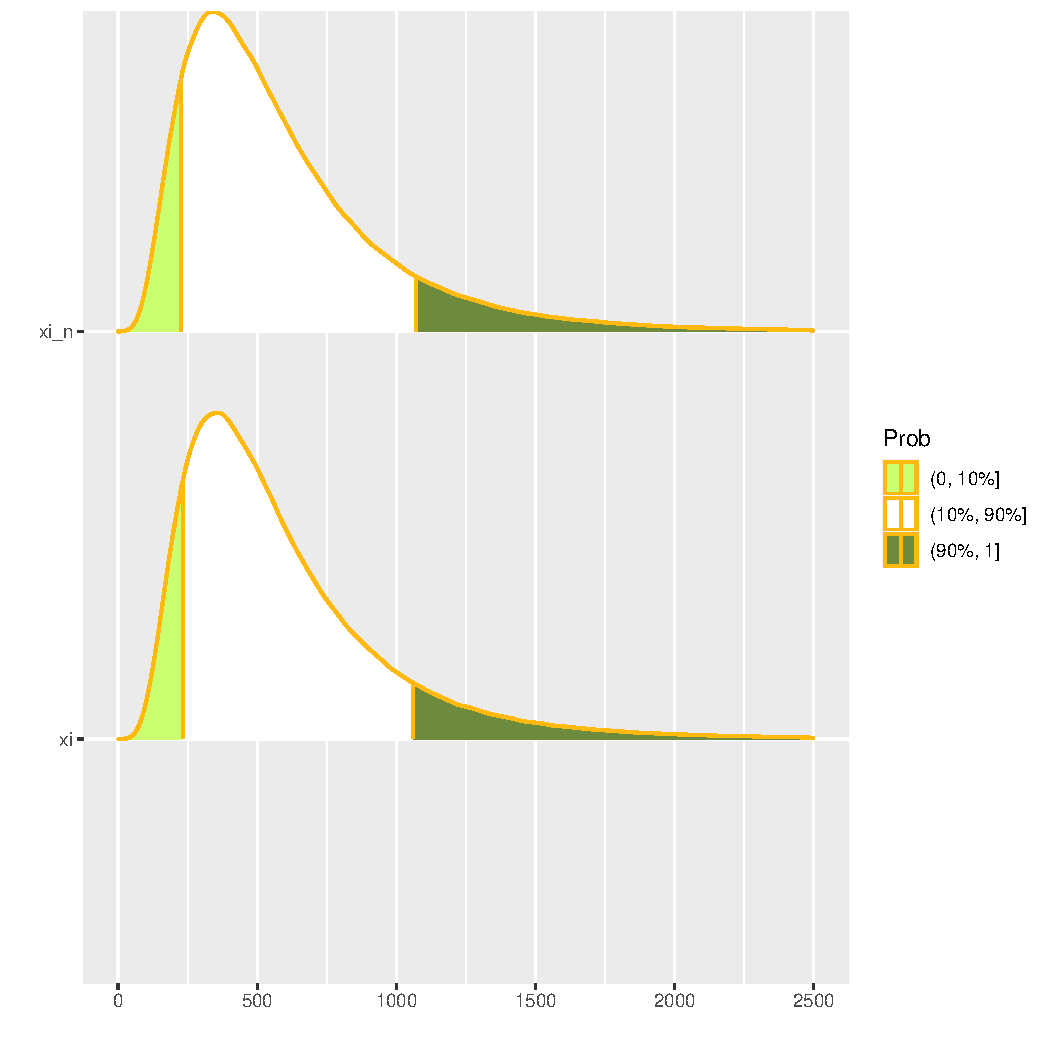
\includegraphics[width=1\linewidth]{img/par_2.pdf}
				\caption{$\sigma_{1}^{2} = 1.05$, $\sigma_{2}^{2} = 0.45$, $err_{med}$ = 0.09\%,  $err_{q_{10}} = 2.4\%$,  $err_{q_{90}} = 1.1\%$. } %% подпись к рисунку
				\label{ris7} %% метка рисунка для ссылки на него
			\end{minipage}
			
		\end{center}
	\end{figure}
	
\end{frame}

\begin{frame}{Часть 5: Сумма двух логнормальных распределений. Точность аппроксимации }
		
	\begin{figure}[h]
		\begin{center}
			\begin{minipage}[h]{0.53\linewidth}
				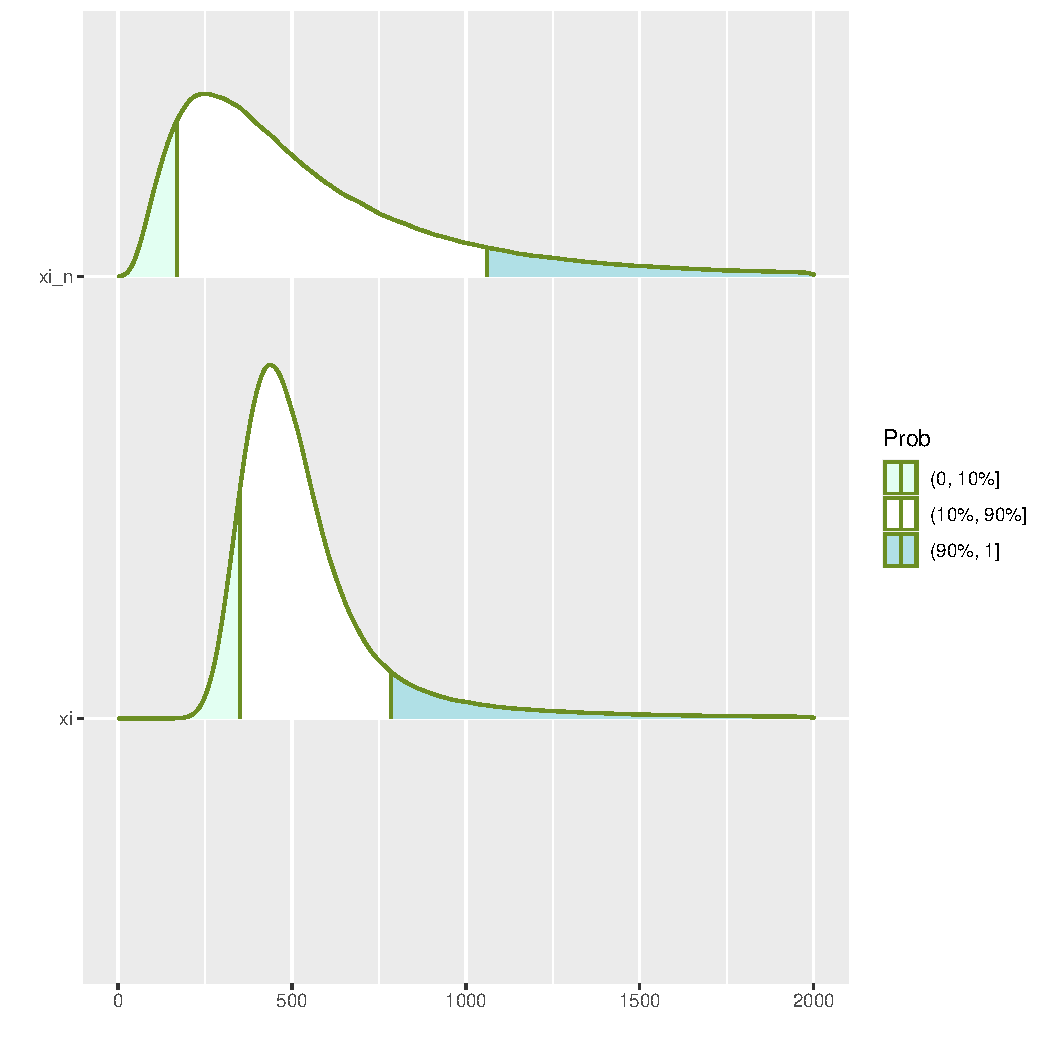
\includegraphics[width=1\linewidth]{img/par_1.pdf}
				\caption{$\sigma_{1}^{2} = 2.25$, $\sigma_{2}^{2} = 0.05$, $err_{med}$ = 9.92\%,  $err_{q_{10}} = 51.34\%$,  $err_{q_{90}} = 39.88\%$. } %% подпись к рисунку
				\label{ris7} %% метка рисунка для ссылки на него
			\end{minipage}
			
		\end{center}
	\end{figure}
\end{frame}
	
\begin{frame}{}
	
	
	\textcolor{blue}{\hbox{\textbf{Мною были получены следующие результаты:}}}
	\begin{enumerate}
		\item Получено условие на $\sigma$ для существования трехточечной симметричной аппроксимации логнормального распределения.
		\item Численно оценена точность аппроксимации мат. ожидания и дисперсии логнормального распределения с помощью метода Свонсона, применяемого к нормальному распределению.
		\item Построен алгоритм для нахождения трехточечной симметричной аппроксимации суммы логнормальных распределений.
		\item Численно оценена точность трехточечной симметричной аппроксимации суммы логнормальных распределений.
	\end{enumerate}
	%\bigskip
	
\end{frame}


	
	
\end{document}